\chapter{车道汇合模型与群决策算法框架}
\section{车道汇合问题模型构建}
道路交汇口广泛存在于城市道路、高速公路中,是一种十分常见的交通场景。交汇的两条道路通常分为主路和辅路。其中主路通常有多条车道,路面较宽敞,车速快;辅路通常只有一条车道,车速较慢。按照我国现行交通法规,辅路车辆应在不影响主路车辆正常通行的情况下汇入主路。在主路车流密集,车速较高时,往往会造成辅路车辆停车等待的情况,带来了道路资源、燃油的浪费。若通过交汇口的车辆均由 CAV 构成,则有可能通过群体性的决策使交汇过程无需停车,同时减小通行时间和燃油损耗。

考虑如图\ref{fig:merge}所示的交汇路口。为了简化问题,考虑主路只有一条车道的情况。可能发生横向碰撞的区域成为交汇区,长度为$S$
。在控制区内,车辆之间、车辆与中央控制器之间允许交换信息并运行控制算法, 控制区起点
到交汇区起点的长度为$L$。
\begin{figure}[htbp]
\centering
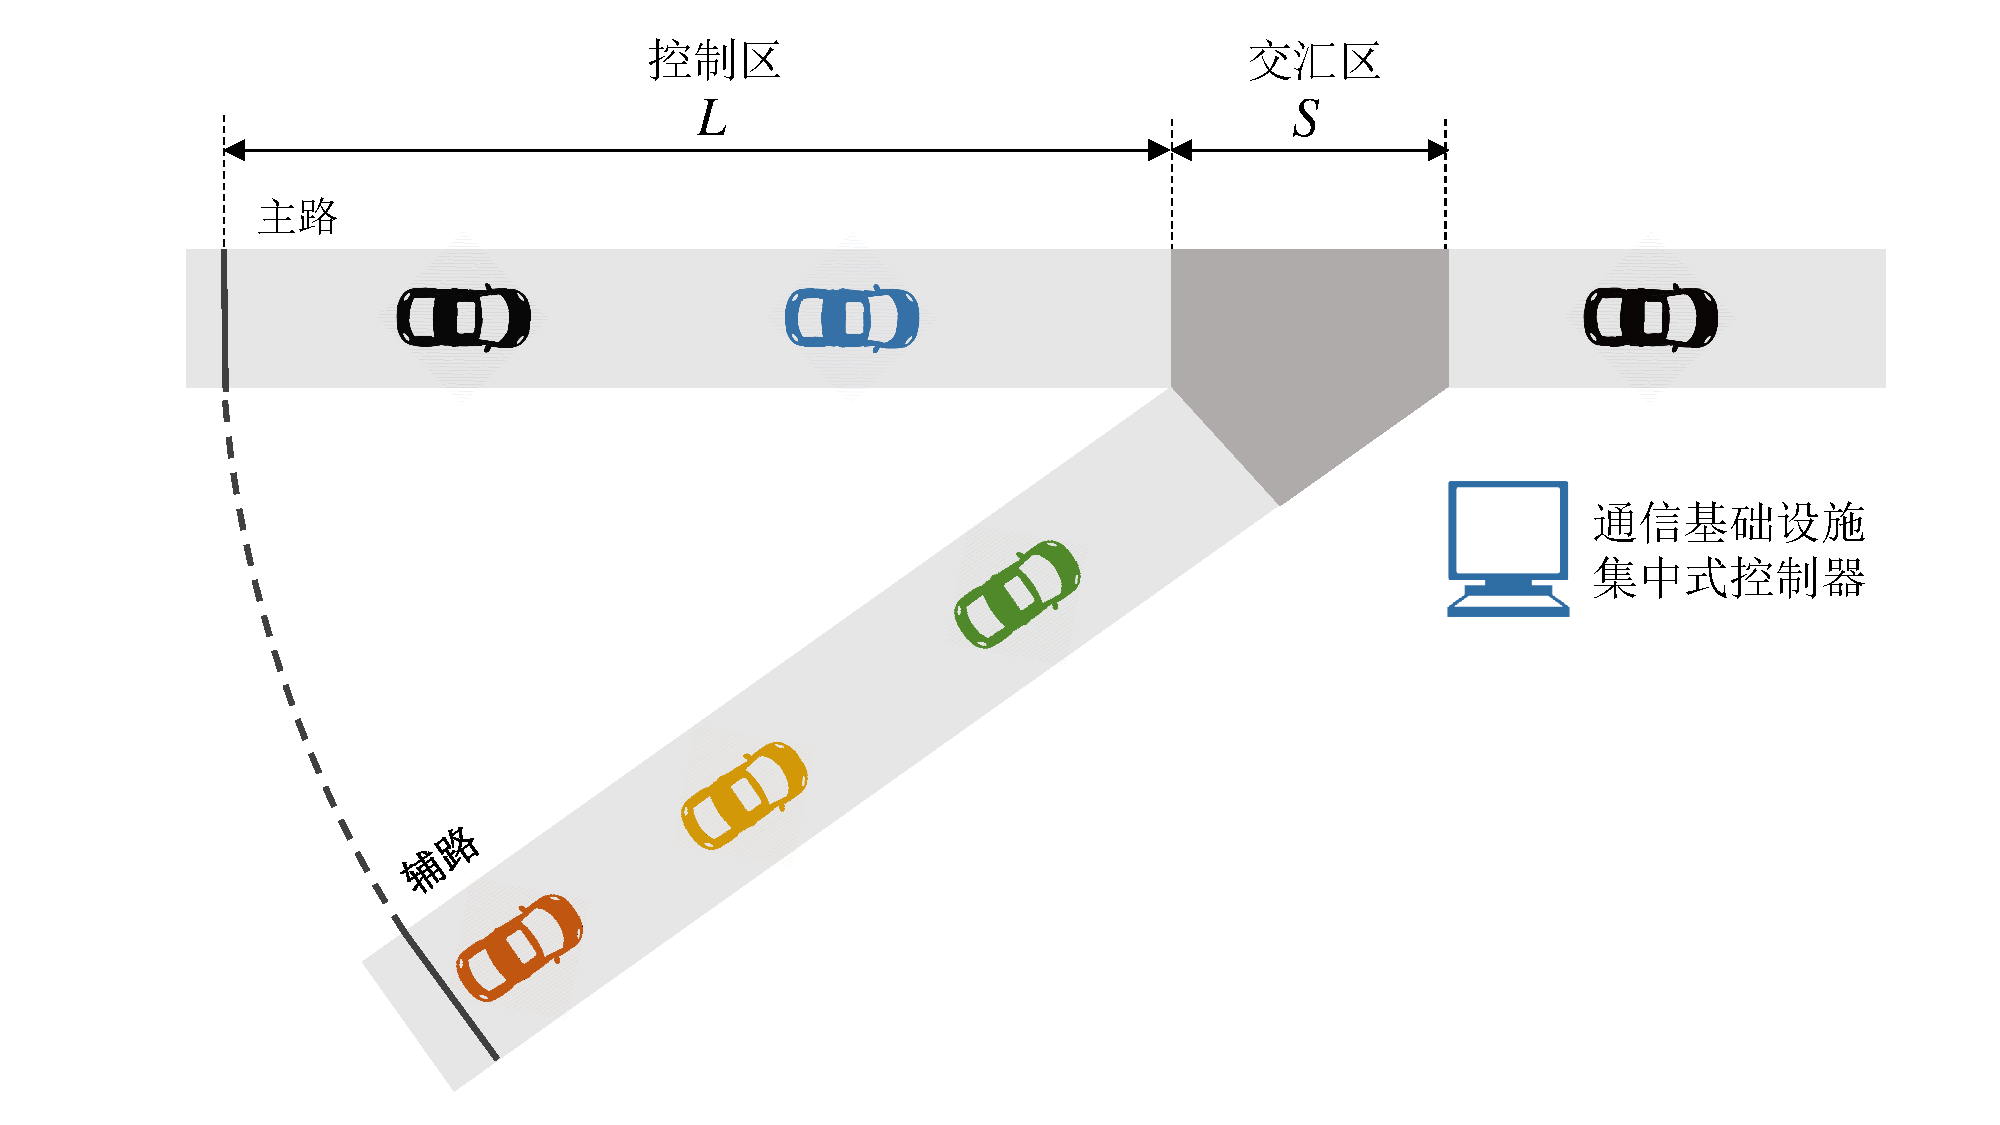
\includegraphics[width=14cm]{../figures/merge.pdf}
\caption{交汇路口示意图}
\label{fig:merge}
\end{figure}

\subsection{车辆状态方程}
假设在时刻 $t$时,位于控制区内的车辆具有某种编号 $\mathcal{N}(t)={1,\dots,N(t)}$,其中 $N(t)$为 $t$时刻控制区内车辆总数。对于每辆车$i\in \mathcal{N}(t)$,系统状态方程为
\begin{equation}
\dot{x}_i=f(t,x_i,u_i),\quad x_i(t_i^0)=x_i^0,
\end{equation}
其中$x_i(t)$,$u_i(t)$分别为第$i$辆车在$t$时刻的状态量和控制量。对于本课题讨论的无人车控制,假定车辆的轨迹已经确定,无需控制方向,只需控制速度。为了保证速度的连续性,选取控制量为加速度,则控制量与状态量的关系为,
\begin{equation}
\begin{gathered}
\dot{p}_i=v_i(t)\\
\dot{v}_i=u_i(t)
\end{gathered}
\end{equation}

其中 $p_i(t)\in \mathcal{P}_i$,$v_i(t)\in \mathcal{V}_i$,$u_i(t)\in \mathcal{U}_i$分别为第 $i$辆车在 $t$时刻的位置,速度和加速度。由于轨迹事先已确定,只需要两个标量 $p_i$与 $v_i$即可确定当前车辆的位置和速度。二者构成了车辆的状态向量 $x_i(t)=[p_i(t), v_i(t)]^\mathrm{T}\in \mathcal{X}_i$,$\mathcal{X}_i=\mathcal{P}\times\mathcal{V}$,并定义进入控制区的初始状态为$x_i^0 = [0, v_i^0]^\mathrm{T}$。

对于实际运行的车辆,其速度和加速度均有限,表达为以下约束,
\begin{equation}
\begin{aligned}
u_{i,\min}\leq u_i(t)\leq u_{i,\max}&, \quad \text{and}\\
0\leq v_{\min}\leq v_i(t)\leq v_{\max}&, \quad \forall t\in[t_i^0, t_i^\mathrm{f}]
\end{aligned}
\label{eq:single_constraint}
\end{equation}
其中 $t_i^\mathrm{f}$为第 $i$辆车离开交汇区的时刻,即控制算法结束的时刻。 $u_{i,\min}$,$u_{i,\max}$分别为第$i$辆车的最小、最大加速度,$v_{\min}$,$v_{\max}$为道路的最低、最高限速。为简单起见,考虑同质车辆,所有CAV均具有相同的最小、最大加速度,即$u_{i,\min}=u_{\min}$,$u_{i,\max}=u_{\max}$。

\subsection{安全性约束与假设}
上一节建立了每辆车的状态方程和单车的约束条件,本节考虑车辆之间的约束关系。

控制算法首先要保证车辆之间不发生追尾。对同一车道上的车辆,定义安全距离$\delta < S$,同车道车辆之间不追尾的约束可以表示为,
\begin{equation}
s_i(t)=p_k(t)-p_i(t)\geq \delta, \ \forall t\in [t_i^0, t_i^\mathrm{f}],
\label{eq:colli_rear}
\end{equation}
其中$k$表示与$i$在同一车道的前一辆车的编号。上式涵盖了控制区、交汇区不发生同车道追尾的约束条件。

车辆仅在交汇区可能与对路车辆发生横向碰撞。给出如下定义:
\begin{definition}
对所有$i\in \mathcal{N}(t)$,定义第 $i$辆车的可能碰撞集 $\Gamma_i$为可能发生横向碰撞的$i$车位置构成的集合,即
\begin{equation}
\Gamma_i\triangleq \{p_i(t)\in[L,L+S],\  \forall t\in [t_i^\mathrm{m},t_i^\mathrm{f}]\}.
\end{equation}
其中$t_i^\mathrm{m}$为第$i$辆车离开控制区,进入交汇区的时刻。
\end{definition}
为了避免横向碰撞,对任意不在同一条路上的两辆车 $\forall i,j\in \mathcal{N}(t)$,给出如下约束:
\begin{equation}
\Gamma_i\cap \Gamma_j=\varnothing, \ \forall t\in [t_i^\mathrm{m},t_i^\mathrm{f}].
\label{eq:colli_lateral}
\end{equation}
上式要求来自相互交汇的两条路上的车辆不能同时出现在交汇区。这个约束必能保证车辆在交汇区不发生横向碰撞,但当交汇区的长度很长时,约束可能过强,没有必要。在下面的章节中将讨论如何放松该约束。

在定义优化目标之前,对控制算法做以下假设。
\begin{assumption}
进入控制区的车$i$满足约束式\ref{eq:single_constraint},\ref{eq:colli_rear}。
\label{ass:restrict}
\end{assumption}
\begin{assumption}
CAV在交汇区保持匀速行驶,且速度相同,即$v_i(t) = v_i(t_i^\mathrm{m}) = v_i(t_i^\mathrm{f}) = v_\mathrm{d}, \ \forall t\in [t_i^\mathrm{m},t_i^\mathrm{f}]$,其中$v_\mathrm{d}$为期望速度。由此可得
\begin{equation}
t_i^\mathrm{f}=t_i^\mathrm{m} + \frac{S}{v_\mathrm{d}}.
\end{equation}
\label{ass:smooth}
\end{assumption}
\begin{assumption}
忽略CAV之间信息传输的延时和错误。
\label{ass:time}
\end{assumption}

在以上假设中,假设\ref{ass:restrict}保证了初始状态的可行性。假设\ref{ass:smooth}忽略了交汇区的速度变化,且假设车辆在进入交汇区之前已经调整到了期望速度$v_\mathrm{d}$。该速度可以根据路段的限速事先给定。这是为了方便讨论交汇区的不碰撞约束,实际情况与此有一定差别。后文将对此展开进一步讨论。假设\ref{ass:time}保证车辆之间信息交互是实时且准确的。但本文的模型在信息的延时和错误处于有限范围内,仍可进行扩展。

\section{群决策算法框架}
% 这里加一段优化目标的综述
\subsection{时间序列的确定}
在假设\ref{ass:smooth}下,考虑到约束式\ref{eq:colli_rear}与式\ref{eq:colli_lateral},可以由$t_{i-1}^\mathrm{m}$确定$t_i^\mathrm{m}$的下界。考虑以下几种情况:
\paragraph{情况一} $i$车与 $i-1$车在同一车道,此时前后车只需保持安全距离,当$i-1$车驶过$\delta$距离后,$i$车便可进入交汇区。由此可得,
\begin{equation}
t_i^\mathrm{m}=t_{i-1}^\mathrm{m} + \frac{\delta}{v_\mathrm{d}}
\end{equation}
\paragraph{情况二}  $i$车与 $i-1$车在不同车道,由式\ref{eq:colli_lateral},当$i-1$车完全驶过交汇区后,$i$车才能进入交汇区。由此可得,
\begin{equation}
t_i^\mathrm{m}=t_{i-1}^\mathrm{m} + \frac{S}{v_\mathrm{d}}
\end{equation}

上述情况二满足了式\ref{eq:colli_lateral}所要求的不同车道不同时出现在交汇区的要求。若交汇区比较长,该要求可以适当放松为,使不同车道间车辆交汇后相距为 $r < S$,$r$为不同车道保证不发生横向碰撞的安全距离。在实际道路条件下,安全距离应随着速度的增加而适当增大。由于交汇区车速仍可视为保持期望速度 $v_\mathrm{d}$,$r$也可以作为常数而预先确定下来。情况二对应的时间关系变为,
\begin{equation}
t_i^\mathrm{m}=t_{i-1}^\mathrm{m} + \frac{r}{v_\mathrm{d}}
\end{equation}

另外,对于不存在前车的第一辆车,其到达交汇区时间 $t_1^\mathrm{m}$可由优化目标解出。这将在下文进一步讨论。

\subsection{优化目标建立}
研究CAV的决策问题,就是在控制量满足一定约束的情况下,对每辆车给出一列控制量输入$u_i(t)$对于车道汇合的场景,一般优化目标包含最小化控制量的输入和最小化平均通行时间。

\subsection{算法可行性论证}
\begin{table}[htb]
  \centering
  \begin{minipage}[t]{0.8\linewidth} % 如果想在表格中使用脚注,minipage是个不错的办法
  \caption[模板文件]{模板文件。如果表格的标题很长,那么在表格索引中就会很不美
    观,所以要像 chapter 那样在前面用中括号写一个简短的标题。这个标题会出现在索
    引中。}
  \label{tab:template-files}
    \begin{tabularx}{\linewidth}{lX}
      \toprule[1.5pt]
      {\heiti 文件名} & {\heiti 描述} \\\midrule[1pt]
      thuthesis.ins & \LaTeX{} 安装文件,\textsc{DocStrip}\footnote{表格中的脚注} \\
      thuthesis.dtx & 所有的一切都在这里面\footnote{再来一个}。\\
      thuthesis.cls & 模板类文件。\\
      thuthesis.cfg & 模板配置文。cls 和 cfg 由前两个文件生成。\\
      thuthesis.bst    & 参考文献 BIB\TeX\ 样式文件。\\
      thuthesis.sty   & 常用的包和命令写在这里,减轻主文件的负担。\\
      \bottomrule[1.5pt]
    \end{tabularx}
  \end{minipage}
\end{table}
\subsection{算法}